%Author Alex Clemmer
%CS 3130 Eng Stats Prob
%Assignment 6:
\documentclass[a4paper]{article}
\usepackage[pdftex]{graphicx}
\usepackage{fancyvrb}
\usepackage{multirow}
\usepackage{amssymb}
\usepackage{amsmath}
\usepackage{haldefs}
\usepackage{fullpage}
\addtolength{\oddsidemargin}{-.05in}
	\addtolength{\evensidemargin}{-.05in}
	\addtolength{\textwidth}{.25in}

	\addtolength{\textheight}{.25in}

\begin{document}

\section*{Assignment 5}
Alex Clemmer\\
Student number: u0458675

\subsection*{Problem 1:} 

\paragraph{(a)} The value I chose for $w$ is $\texttt{aaaaaabbbbbbaaaaaabbbbbb}$.

\paragraph{(b)} The value I chose for $i$ is $\texttt{2}$.

\paragraph{(c)} For $L= \{ww : w \in \{a,b\}^*\}$ and $w = a^n b^n a^n b^n$, there is absolutely no way that we could pick some part of $w$ such that pumping it would give us a string inside $L$. Consider $w=uvxyz$. We can only pump $v$ and $y$, so no matter what we choose for each division of $w$, we will always end up doubling either part of the string, and not another part of the string such that it excludes the string from $L$, or we end up doubling the entire string, which gives us a string that is also not in $L$.

The reason this is that doubling only two of the composing variables will allow us to either double only 2 of the 4 variables (e.g., $w = a^n b^i a^i b^n : i \neq n$), or else we end up doubling two types of character at once, giving us too many characters to be in $L$, (e.g., $w = a^n b^n a^n b^n a^n b^n$).

Here are some examples: if $v= aaa$ from the second set of $a$'s, and $y=bbb$ from the second set of $b$'s, then pumping gives us $w = a^n b^i a^i b^n : i \neq n$, and thus it is not in $L$. If $v = a^n b^n$ and $y= a^n b^n$, pumping gives us $w= a^n b^n a^n b^n  a^n b^n  a^n b^n$, which is also not in $L$. As you can see if 

\subsection*{Problem 2:} 

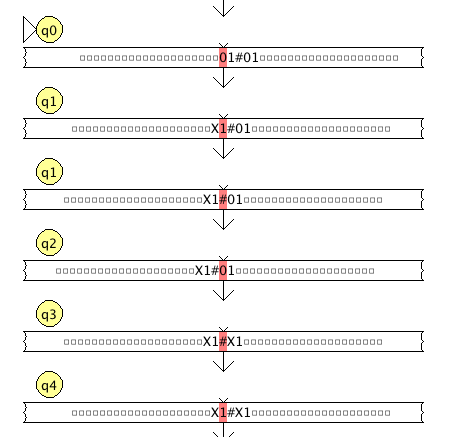
\includegraphics[scale=0.50]{p2_trace.png}

\subsection*{Problem 3:}

We freeze in two places. First, on step 2: \\

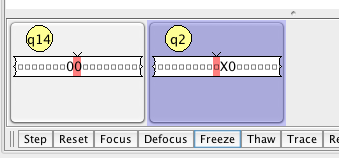
\includegraphics[scale=0.50]{freeze_step_2.png} \\

...and second, on step 3: \\

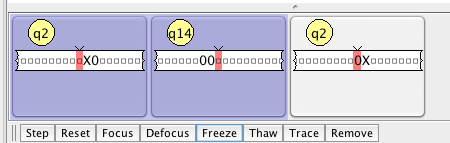
\includegraphics[scale=0.50]{freeze_step_3.png} \\

And here's the trace: \\

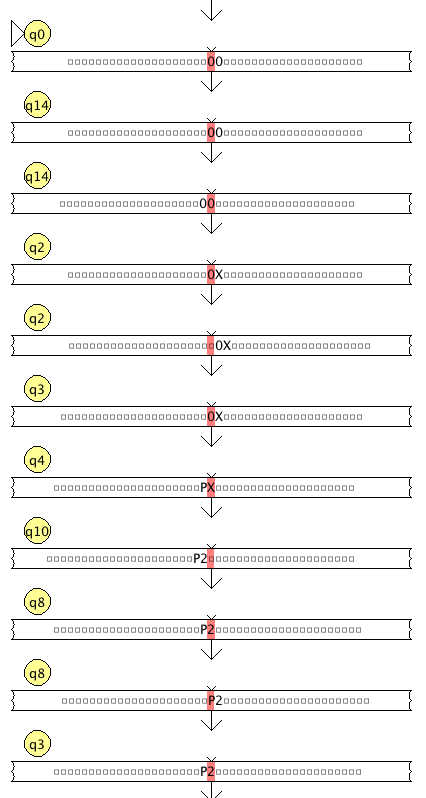
\includegraphics[scale=0.50]{p3_trace.png}

\subsection*{Problem 4:}

This TM accepts all strings with the substring $\texttt{0101}$.

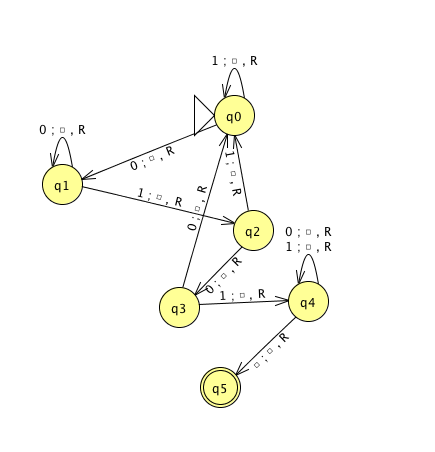
\includegraphics[scale=0.6]{p4_TM.png}

The required test is as follows; there are more tests included, but the one you're looking for is the very last one. \\

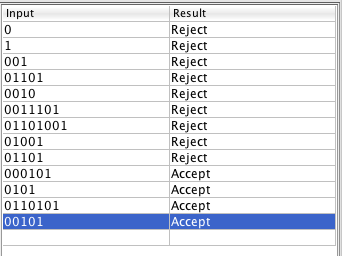
\includegraphics[scale=0.6]{p4_validation.png}

\subsection*{Problem 5:}

The TM and tests are below:

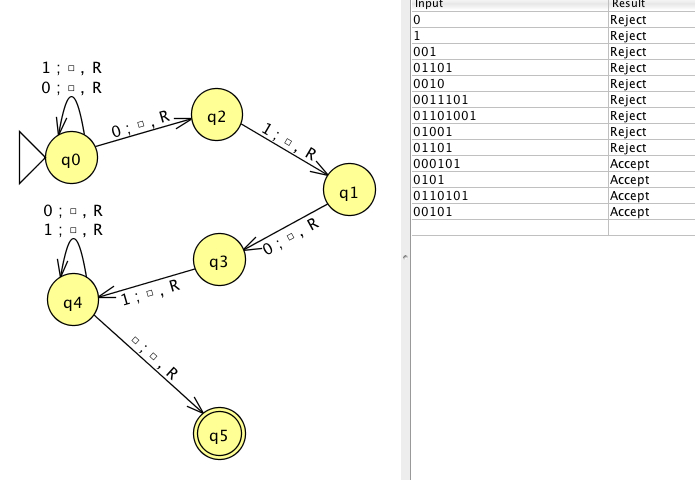
\includegraphics[scale=0.4]{p5_tm_and_trace.png} \\

Below is the picture of all the paths that would lead to rejection (and were thus frozen), along with the one path that would lead to accept. They were frozen at 2nd and 5th steps, respectively. \\

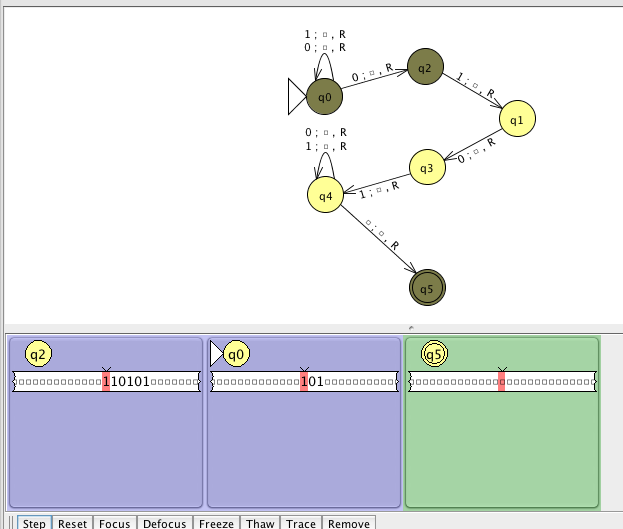
\includegraphics[scale=0.4]{p5_freeze.png} \\

\subsection*{Problem 6:}

\paragraph{(a)} The language $L = \{0^n 1^n | n \ge 0 \}$ is a problem we've faced repeatedly in the course. It is a CFL; since TMs can recognize any CFL, it is clearly recursively enumerable. To recognize this string, we need only one stack, the TM need only count the number of 0s and repeatedly pop the count when it reaches the 1s. At the end, there should be both an empty stack and a consumed string.

It turns out that this language is also recursive. In order to recognize all strings not in $L$, all we need to do is look for every type of string that is $\textit{not}$ in $L$. This rule is not hard in principle, but it does require some careful attention to exceptions and corner cases. You would check, for example, strings where 0 and 1 are not in that order, where there's different numbers of each, where they both occur more than once (e.g., 0101010, rather than $0^n 1^n$), and so on.

Since both the original CFL and its complement can be emulated by a TM, they will always cause the TM to halt, and thus the language again is recursive.

\paragraph{(b)} This is also recursive. Any language representable by a regular expression is a regular language, which can be emulated with a TM. If you're wondering, one example of a regex that fulfills these criteria is $L = (01)^*$, which is recursive, and also has an infinite number of strings. Again, since this is an RL, all the TM needs to do is emulate the FA that describes this regex.

Also, since RLs are closed over the complement operation, all the above will hold for its inverse. Thus, the TM will halt in every case, whether it accepts or not. The language is therefore recursive.

\paragraph{(c)} We can simply invoke our TM on some TM; if we run the string end in an accept state, then that machine is in the language. If it halts and does not accept, it's not in the language. The only time we run into a problem is when we ask if some arbitrary machine over an infinite domain $\textit{doesn't}$ halt: if we invoke some TM on some string $w$ and the result is that the TM loops, then the simulation will never stop.

The complement is all the string that do NOT include the substring. Since this is again enumerable by an RL, and we've established the concept as it relates to TMs above, the complement clearly is RE, which makes the relationship recursive.

\paragraph{(d)} Recursive. A TM can simulate some arbitrary TM. Since here the stipulation is that the TMs we are accepting also accepts the string $\texttt{0101}$, we know they represent a regular language, and thus will halt for all finite input. Since these TMs represent an RL, they are also closed over inversion, and their complements will thus also halt over any finite. Thus we know that this language is also recursive.

\paragraph{(e)} This language consists essentially of all TMs: any possible TM will either accept, reject, or loop over the string $\texttt{0101}$. The set of all TMs is RE, but it is not recursive, because we do not know that it halts over all elements in the language (and in fact for some, definitely won't).

\paragraph{(f)} Both the number of CFGs and regular expressions that have $\texttt{0101}$ are infinite. Important also is that we know that the regular expression is not infinite, as it is representative of a regular language. Also, RLs are invertible, so that part of the equation is for sure recursive.

What is slightly more tricky is the CFG. CFGs are not closed over inversion, so we have no guarantee that the CFGs in this set are recursive. So it's only RE.

\subsection*{Problem 7:}

$L(P) = \{ L(N) | L(M) \}$



\end{document}